
\chapter[Lý thuyết: Hiện tượng giao thoa sóng và các điều kiện xảy ra giao thoa sóng cơ]{Lý thuyết: Hiện tượng giao thoa sóng và các điều kiện xảy ra giao thoa sóng cơ}
\section{Lý thuyết}
\subsection{Định nghĩa}

\begin{itemize}
	\item 
	Hai nguồn kết hợp là hai nguồn dao động \bltext{cùng} phương, \bltext{cùng} chu kì (hay tần số) và có hiệu số pha \bltext{không đổi theo thời gian}. Hai nguồn kết hợp có cùng pha là hai nguồn đồng bộ.
	\item
	Hai sóng do hai nguồn kết hợp phát ra là hai sóng \bltext{kết hợp}.
	\item 
	Hiện tượng giao thoa là hiện tượng hai sóng \bltext{kết hợp} khi gặp nhau thì có những điểm ở đó chúng luôn \bltext{tăng cường} lẫn nhau, có những điểm ở đó chúng luôn \bltext{triệt tiêu} nhau.
\end{itemize}
\begin{center}
	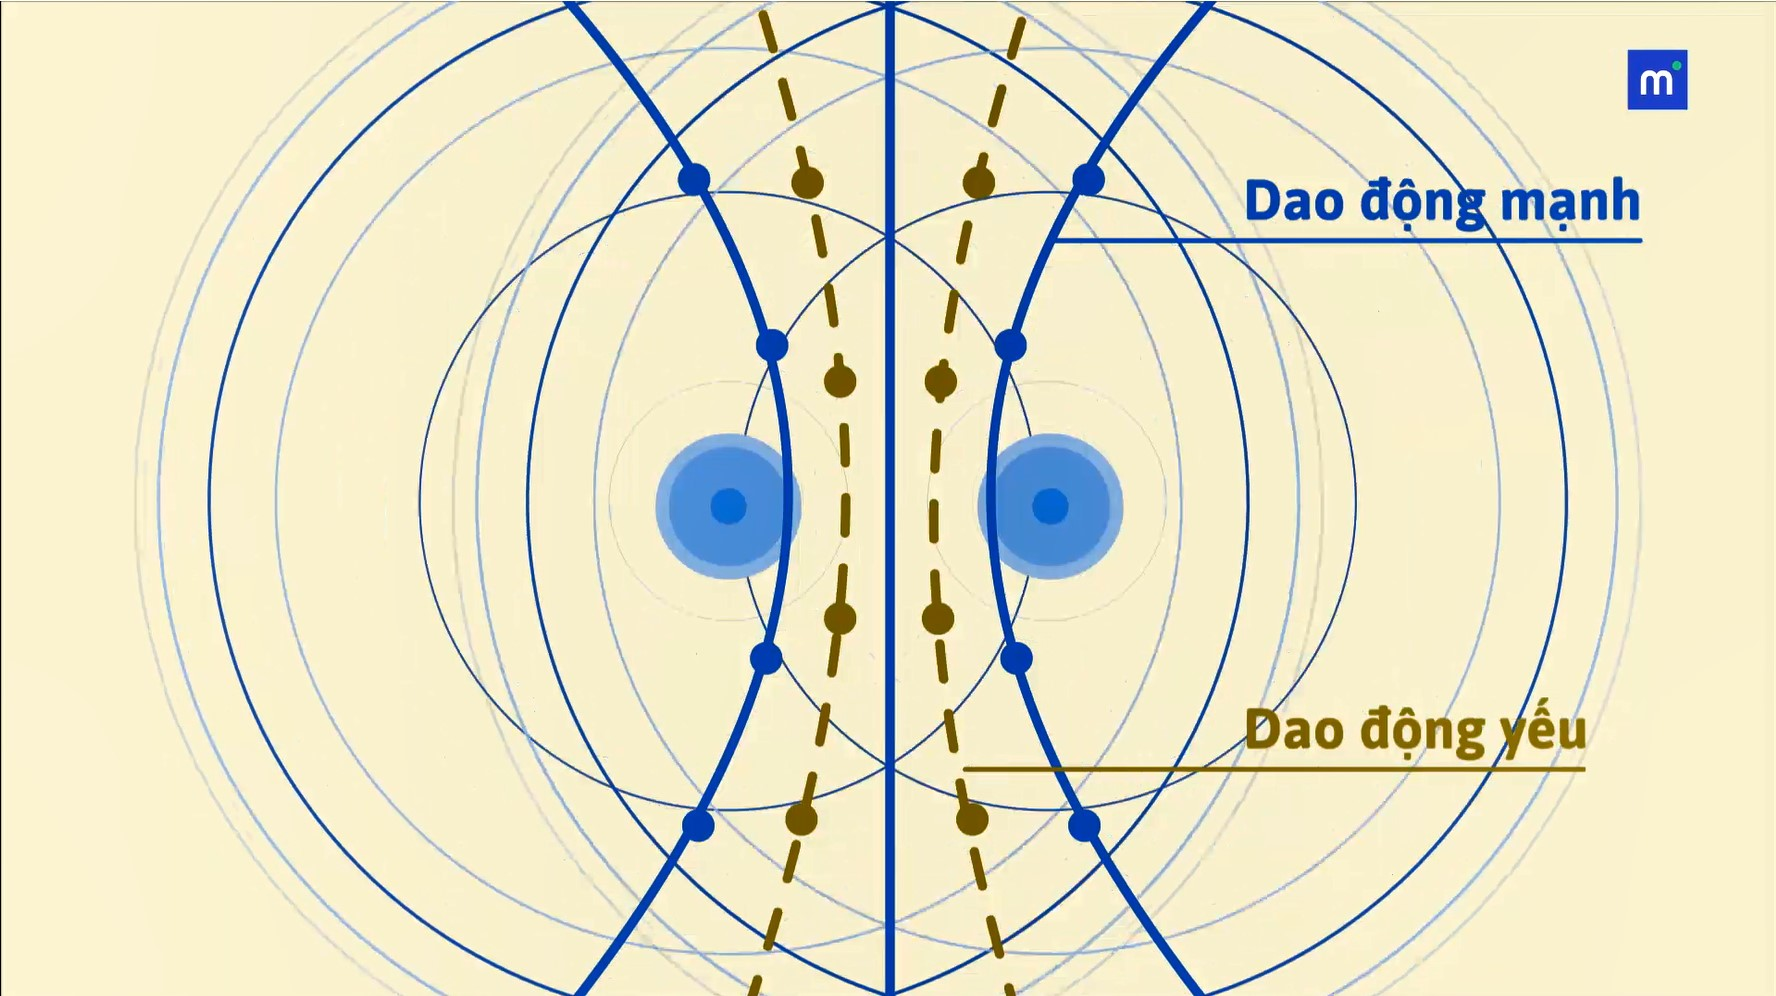
\includegraphics[scale=0.3]{../figs/VN12-PH-11-L-006-1-V2-1.jpg}
\end{center}
\subsection{Phương trình dao động của một điểm trên vùng giao thoa}

\begin{itemize}
	\item Xét hai nguồn kết hợp $\text{S}_1$, $\text{S}_2$ có phương trình dao động lần lượt là 
	\begin{equation*}
		u_{\text{S}_1} = a \cos (\omega t + \varphi_1),
	\end{equation*}
	\begin{equation*}
		u_{\text{S}_2} = a \cos (\omega t + \varphi_2).
	\end{equation*}
	\item Gọi M là một điểm nằm trong vùng giao thoa giữa hai nguồn, cách nguồn $\text{S}_1$ một khoảng $d_1$, cách nguồn $\text{S}_2$ một khoảng $d_2$. 
	
	+ Phương trình sóng tại M do $\text{S}_1$ truyền tới là 
	\begin{equation*}
		u_{\text{M}_1} = a \cos \left(\omega t + \varphi_1 -\dfrac{2\pi d_1}{\lambda}\right),
	\end{equation*}
	+ Phương trình sóng tại M do $\text{S}_2$ truyền tới là 
	\begin{equation*}
		u_{\text{M}_2} = a \cos \left(\omega t + \varphi_2 -\dfrac{2\pi d_2}{\lambda}\right).
	\end{equation*}
	+ Phương trình sóng tổng hợp tại M là
	\begin{equation*}
		u_{\text{M}}=u_{\text{M}_1} + u_{\text{M}_2} = a \cos \left(\omega t + \varphi_1 -\dfrac{2\pi d_1}{\lambda}\right)+ a \cos \left(\omega t + \varphi_2 -\dfrac{2\pi d_2}{\lambda}\right), 
	\end{equation*}
	suy ra
	\begin{equation*}
		u_{\text{M}} = 2a \cos \left(\dfrac{\varphi_1 - \varphi_2}{2} + \dfrac{\pi (d_2-d_1)}{\lambda}\right) \cdot  \cos \left(\omega t +\dfrac{\varphi_1 + \varphi_2}{2} - \dfrac{\pi (d_1+d_2)}{\lambda}\right).
	\end{equation*}
	\item  Dao động của phần tử tại M là dao động điều hòa, cùng tần số với hai nguồn có biên độ dao động là
	\begin{equation*}
		A_{\text{M}} = 2a\left|\cos \left(\dfrac{\varphi_1 - \varphi_2}{2} + \dfrac{\pi (d_2-d_1)}{\lambda}\right)\right|.
	\end{equation*}
	Trường hợp hay gặp nhất là hai nguồn cùng pha, tức là $|\varphi_1 - \varphi_2| =k2\pi$, khi đó 
	\begin{equation*}
		A_{\text{M}} = 2a\left|\cos \left(\dfrac{\pi (d_2-d_1)}{\lambda}\right)\right|.
	\end{equation*}
\end{itemize}
\section{Mục tiêu bài học - Ví dụ minh họa}
\begin{dang}{Mô tả được hiện tượng giao thoa\\ của hai sóng}
	\viduii{1}{Chọn phát biểu chính xác nhất. Hiện tượng giao thoa sóng là
		\begin{mcq}
			\item hiện tượng hai sóng kết hợp khi gặp nhau thì có những điểm ở đó chúng luôn tăng cường lẫn nhau.
			\item hiện tượng hai sóng kết hợp khi gặp nhau thì có những điểm ở đó chúng luôn triệt tiêu nhau.
			\item hiện tượng hai sóng kết hợp khi gặp nhau thì có những điểm ở đó chúng luôn tăng cường lẫn nhau, có những điểm ở đó chúng luôn triệt tiêu nhau.
			\item hiện tượng hai sóng bất kì gặp nhau.
		\end{mcq}
	}
	{
		\begin{center}
			\textbf{Hướng dẫn giải}
		\end{center}
		
		Hiện tượng giao thoa sóng là hiện tượng hai sóng kết hợp khi gặp nhau thì có những điểm ở đó chúng luôn tăng cường lẫn nhau, có những điểm ở đó chúng luôn triệt tiêu nhau.
		
		
		\textbf{Đáp án: C}.
	}
	
	\viduii{1}
	{
		Điều kiện để có giao thoa sóng là gì?
		\begin{mcq}
			\item Có hai sóng chuyển động ngược chiều giao nhau.
			\item Có hai sóng cùng tần số và có độ lệch pha không đổi.
			\item Có hai sóng cùng bước sóng giao nhau.
			\item Có hai sóng cùng biên độ, cùng tốc độ giao nhau.
		\end{mcq}
	}{
		\begin{center}
			\textbf{Hướng dẫn giải}
		\end{center}
		
		Điều kiện có giao thoa sóng là: Hai sóng là hai sóng kết hợp tức là hai sóng cùng tần số và có độ lệch pha không đổi theo thời gian (hoặc hai sóng cùng pha).
		
		\textbf{Đáp án: B.}
	}
	
\end{dang}
\begin{dang}{Xây dựng được phương trình\\ giao thoa sóng cơ}
	\viduii{3}{Tại hai điểm A, B trên mặt nước có hai nguồn dao động theo phương thẳng đứng với phương trình $u_{\text{A}}= u_{\text{B}} = 3 \cos 20 \pi t\ \text{cm}$, tốc độ truyền sóng $v=6\ \text{m/s}.$ Viết phương trình sóng tại điểm M cách A đoạn $15\ \text{cm}$, cách B đoạn $20\ \text{cm}$.
	}
	{
		\begin{center}
			\textbf{Hướng dẫn giải}
		\end{center}
		
		\begin{itemize}
			\item Tần số của sóng:
			\begin{equation*}
				f=\dfrac{\omega}{2\pi} = 10\ \text{Hz}.
			\end{equation*}
			\item Bước sóng:
			\begin{equation*}
				\lambda = \dfrac{v}{f} = 60\ \text{cm}.
			\end{equation*}
			\item Phương trình sóng tại M:
			\begin{equation*}
				u_{\text{M}}=2a \cos \left(\dfrac{\varphi_1 - \varphi_2}{2} + \dfrac{\pi (d_2-d_1)}{\lambda}\right) \cdot  \cos \left(\omega t +\dfrac{\varphi_1 + \varphi_2}{2} - \dfrac{\pi (d_1+d_2)}{2\lambda}\right).
			\end{equation*}
			\item Thay số vào $u_{\text{M}}$ 
			\begin{equation*}
				u_{\text{M}}= 2 \cdot 3 \cos \left(0 + \dfrac{\pi (15-20)}{60}\right) \cdot  \cos \left(20\pi t + 0 - \dfrac{\pi (15+20)}{\lambda}\right),
			\end{equation*}
			suy ra 
			\begin{equation*}
				u_{\text{M}}= 6 \cos \left(-\dfrac{\pi}{12}\right) \cos \left(20\pi t - \dfrac{7\pi}{12}\right).
			\end{equation*}
		\end{itemize} 
	}
	
	\viduii{3}
	{
		Hai mũi nhọn S$_1$S$_2$ cách nhau 9 cm, gắn ở đầu một cần rung có tần số $f=\SI{100}{Hz}$ được đặt cho chạm nhẹ vào một chất lỏng. Vận tốc truyền sóng trên mặt chất lỏng là $v=\text{0,8}\ \text{m/s}$. Gõ nhẹ cho cần rung thì 2 điểm S$_1$S$_2$ dao động theo phương thẳng đứng với phương trình dạng $u=a\cos 2\pi ft$. Điểm M trên mặt chất lỏng cách đều và dao động cùng pha S$_1$S$_2$ gần S$_1$S$_2$ nhất có phương trình dao động là
		\begin{mcq}(2)
			\item $u_\text{M} = a\cos (200\omega t + 20\pi)$.
			\item $u_\text{M} = 2a\cos (200\pi t - 12\pi)$.
			\item $u_\text{M} = 2a\cos (200\omega t - 10\pi)$.
			\item $u_\text{M} = a\cos (200\pi t )$.
		\end{mcq}
	}{
		\begin{center}
			\textbf{Hướng dẫn giải}
		\end{center}
		
		Bước sóng:
		
		\begin{equation*}
			\lambda =\dfrac{v}{f} = \SI{0,8}{cm}.
		\end{equation*}
		
		Tốc độ góc:
		
		\begin{equation*}
			\omega = 2\pi f = 200\pi\ \text{rad/s}.
		\end{equation*}
		
		M cách đều hai nguồn nên M nằm trên đường trung trực của S$_1$S$_2$ lúc này $d_1=d_2 = D$.
		
		Phương trình giao thoa sóng tại M: 
		
		\begin{equation*}
			u_\text{M} = 2u_0 \cos \dfrac{\pi(d_2-d_1)}{\lambda} \cdot \cos \left (\omega t -\dfrac{\pi(d_2-d_1)}{\lambda}\right).
		\end{equation*}
		
		Vì $d_1=d_2=d$.	Suy ra
		
		\begin{equation*}
			u_\text{M} = 2u_0 \cos \left(\omega t -\dfrac{2\pi d}{\lambda}\right).
		\end{equation*}
		
		Để M cùng pha với nguồn thì $\dfrac{2\pi d}{\lambda} =k2\pi$. 
		
		\begin{equation*}
			\Rightarrow k =\dfrac{d}{\lambda} = \text{5,625}.
		\end{equation*}
		
		Vì M gần S$_1$S$_2$ nhất nên $k=6$. Phương trình tại M là
		
		\begin{equation*}
			u_\text{M} = 2a\cos (200\pi t - 12\pi).
		\end{equation*}
		
		\textbf{Đáp án: B.}
	}
	
\end{dang}